\chapter{Methods}
\section{Dataset}
The datset was created by Dr. Tichy and his team in the Computer Vision Annotation Tool (CVAT). It was extended and improved multiple times over the course of this work and there is still ongiong work on it. At the time of writing this report it consisted of 2599 bitewing X-ray images with 4575 annotations of tooth decay. There are 890 images withou any decay. The distribution of dental caries per image is depicted in the figure \ref{fig:hist_caries_per_img}, for the clarity reasions we omited 6 images, which contained more than 10 caries. From the histogram on the figure \ref{fig:hist_caries_dim} we obseve, that most of the caries have dimensions between 10 and 75 pixels, but there are outliers, that are as big as 380 pixels per dimension. This diversity is increasing the difficulty of the task.

We used the COCO data-format to store the data and used the format during the whole work only with rare exceptions, when custom data-format was needed. During the experiments we used the 70:15:15 split into training, validation and test dataset.
\begin{figure}
    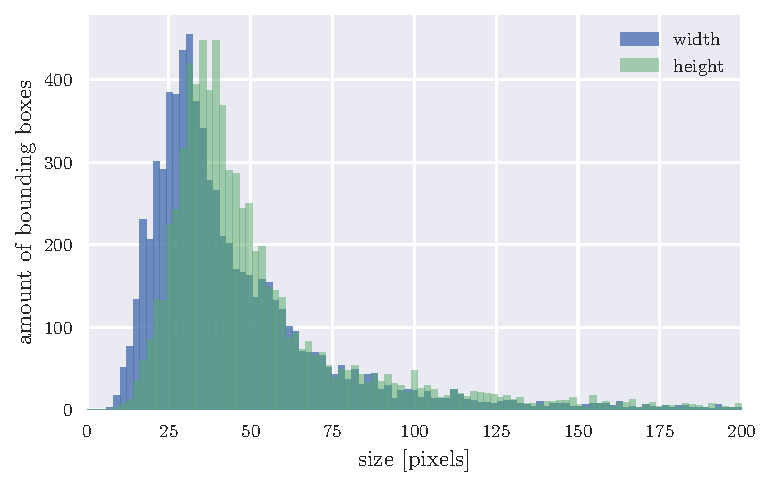
\includegraphics[width = \linewidth]{images/dataset_histogram.pdf}
    \caption{Histogram of bonding boxes dimensions in the dataset}
    \label{fig:hist_caries_dim}
\end{figure}

\begin{figure}
    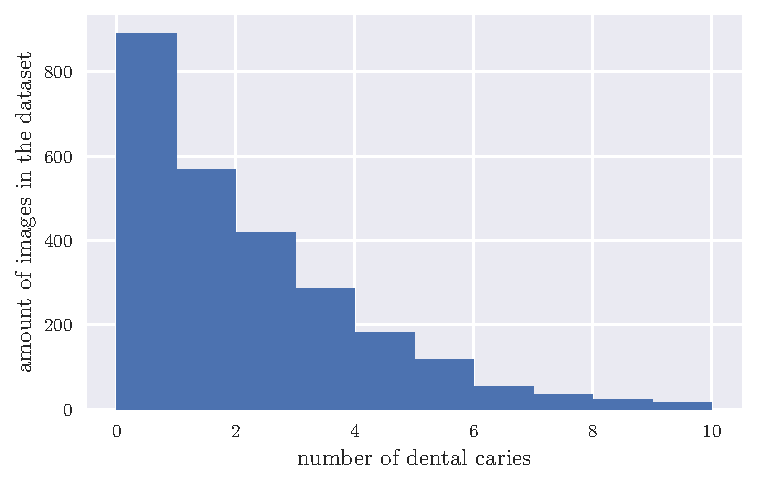
\includegraphics[width=\linewidth]{images/caries_histogram.pdf}
    \caption{Histogram of the amount of dental caries per image}
    \label{fig:hist_caries_per_img}
\end{figure}

\section{Neural network models}